\subsection{wait statuses}

\begin{frame}[fragile,label=exitStatuses]{exit statuses}
\begin{lstlisting}[
    language=C++,
    moredelim={**[is][\btHL<1-|handout:1->]{@1}{1@}},
]
int main() {
    return @101@;  /* or exit(0);  */
}
\end{lstlisting}
\end{frame}

\begin{frame}[fragile,label=extractStatus]{the status}
\begin{lstlisting}[
    language=C++,
    style=smaller,
    moredelim={**[is][\btHL<2|handout:0>]{@2}{2@}},
]
#include <sys/wait.h>
...
  waitpid(child_pid, &status, 0);
  if (@2WIFEXITED(status)2@) {
    printf("main returned or exit called with %d\n",
           @2WEXITSTATUS(status)2@);
  } else if (WIFSIGNALED(status)) {
    printf("killed by signal %d\n", WTERMSIG(status));
  } else {
      ...
  }
\end{lstlisting}
``status code'' encodes \myemph{both return value and if exit was abnormal} \\
W* macros to decode it
\end{frame}


\section{shells}

\subsection{shells, the concept}

\begin{frame}{shell}
\begin{itemize}
    \item allow user (= person at keyboard) to run applications
    \item user's wrapper around process-management functions
\end{itemize}
\end{frame}

\begin{frame}{aside: shell forms}
\begin{itemize}
    \item POSIX: command line you have used before
        \vspace{.5cm}
    \item also: graphical shells
        \begin{itemize}
        \item e.g. OS X Finder, Windows explorer
        \end{itemize}
    \item other types of command lines?
    \item completely different interfaces?
\end{itemize}
\end{frame}



\subsection{searching for programs}
%\againframe<2>{commandLineFeatures}

\begin{frame}[fragile,label=searchForPrograms]{searching for programs}
\begin{itemize}
    \item POSIX convention: PATH \textit{environment variable}
        \begin{itemize}
        \item example: \texttt{/home/cr4bd/bin:/usr/bin:/bin} 
        \item list of directories to check in order
        \end{itemize}
    \item environment variables = key/value pairs stored with process
        \begin{itemize}
        \item by default, left unchanged on execve, fork, etc.
        \end{itemize}
    \item one way to implement:  [pseudocode]
\begin{lstlisting}
for (directory in path) {
    execv(directory + "/" + program_name, argv);
}
\end{lstlisting}
\end{itemize}
\end{frame}


\subsection{kernel buffering}

\usetikzlibrary{arrows.meta,chains,shapes}

\begin{frame}{kernel buffering (reads)}
\begin{tikzpicture}
\tikzset{
    >=Latex,
    component box/.style={draw,thick,minimum width=10cm,minimum height=1cm,align=center},
    component box big/.style={component box,minimum height=2.5cm},
    component box small/.style={component box,minimum width=4cm},
    subcomponent box/.style={draw,thick,minimum width=2cm,align=center,font=\small},
    event line/.style={draw,ultra thick},
    event box/.style={draw,thick,fill=white,inner sep=0.25mm,font=\small, align=center},
    number box A/.style={draw=blue,thick,fill=blue!10,ellipse,font=\small,inner sep=0.1mm},
    number box A alt/.style={draw=blue,thick,dotted,fill=blue!5,ellipse,font=\small,inner sep=0.1mm,
            alt=<4>{draw=red,fill=red!10}},
    number box B/.style={draw=green,thick,fill=green!10,ellipse,font=\small,inner sep=0.1mm},
}
\node[component box] (process) {program};
\node[component box big,anchor=north] (os) at ([yshift=-2cm]process.south) {operating system \\ ~ \\ ~};
\node[component box small,anchor=north east] (keyboard) at ([xshift=-.5cm,yshift=-1.5cm]os.south) {keyboard};
\node[component box small,anchor=north west] (disk) at ([xshift=.5cm,yshift=-1.5cm]os.south) {disk};
\begin{visibleenv}<2->
\draw[event line,->] (keyboard.north) -- (os.south -| keyboard.north) node[midway,event box] (kp event){keypress happens, read};
\node[number box A,anchor=east] (kp event number) at (kp event.north west) {1};
\begin{visibleenv}<4->
    \node[number box A alt,anchor=east] at ([xshift=-.5cm,yshift=.1cm]kp event number.west) {2};
    \node[font=\small,anchor=east,inner sep=0.25mm] at (kp event number.west) {or};
\end{visibleenv}
\node[anchor=south,subcomponent box] (keyboard buffer)  at (os.south -| keyboard.north) {buffer: keyboard input \\ waiting for program};
\end{visibleenv}
\begin{visibleenv}<3->
    \draw[event line,->] ([xshift=-4cm]process.south) -- ([xshift=-4cm]os.north) node[midway,event box,xshift=-1cm] (read ev) {read char \\ from terminal};
\node[number box A,anchor=east] (read ev number) at (read ev.north west) {2};
\begin{visibleenv}<4->
    \node[number box A alt,anchor=east] at ([xshift=-.5cm,yshift=.1cm]read ev number.west) {1};
    \node[font=\small,anchor=east,inner sep=0.25mm] at (read ev number.west) {or};
\end{visibleenv}
    \draw[event line,<-] ([xshift=-2cm]process.south) -- ([xshift=-2cm]os.north) node[midway,event box,xshift=-.5cm] (from buf ev) {\ldots via buffer};
\node[number box A,anchor=east] at (from buf ev.north west) {3};
\end{visibleenv}
\begin{visibleenv}<5->
\draw[event line,->] ([xshift=1cm]process.south) -- ([xshift=1cm]os.north) node[midway,event box,xshift=0cm] (read file ev)  {read char \\ from file};
\node[number box B,anchor=east] at (read file ev.north west) {1};
\end{visibleenv}
\begin{visibleenv}<6->
\draw[event line,->] (disk.north) -- (os.south -| disk.north) node[midway,event box] (xfer disk ev) {read \textit{block} of data from disk};
\node[number box B,anchor=east] at (xfer disk ev.north west) {2};
\node[anchor=south,subcomponent box] at (os.south -| disk.north) {buffer: recently read \\ data from disk};
    \draw[event line,<-] ([xshift=4cm]process.south) -- ([xshift=4cm]os.north) node[midway,event box,xshift=0cm] (from disk buffer ev) {\ldots via buffer};
\node[number box B,anchor=east] at (from disk buffer ev.north west) {3};
\end{visibleenv}
\end{tikzpicture}
\end{frame}

\begin{frame}{kernel buffering (writes)}
\begin{tikzpicture}
\tikzset{
    >=Latex,
    component box/.style={draw,thick,minimum width=10cm,minimum height=1cm,align=center},
    component box big/.style={component box,minimum height=2.25cm},
    component box small/.style={component box,minimum width=4cm},
    subcomponent box/.style={draw,thick,minimum width=2cm,align=center,font=\small},
    event line/.style={draw,ultra thick},
    event box/.style={draw,thick,fill=white,inner sep=0.25mm,font=\small, align=center},
}
\node[component box] (process) {program};
\node[component box big,anchor=north] (os) at ([yshift=-2cm]process.south) {operating system \\ ~ \\ ~};
\node[component box small,anchor=north east] (network) at ([xshift=-.5cm,yshift=-1.5cm]os.south) {network};
\node[component box small,anchor=north west] (disk) at ([xshift=.5cm,yshift=-1.5cm]os.south) {disk};
\begin{visibleenv}<3->
\draw[event line,<-] (keyboard.north) -- (os.south -| keyboard.north) node[midway,event box] {(when ready) \\ send data};
\node[anchor=south,subcomponent box] (keyboard buffer)  at (os.south -| keyboard.north) {buffer: output \\ waiting for network};
\end{visibleenv}
\begin{visibleenv}<2->
\draw[event line,->] ([xshift=-4cm]process.south) -- ([xshift=-4cm]os.north) node[midway,event box,xshift=0cm] {print char \\ to remote machine};
\end{visibleenv}
\begin{visibleenv}<4->
\draw[event line,->] ([xshift=1cm]process.south) -- ([xshift=1cm]os.north) node[midway,event box,xshift=0cm] {write char \\ to file};
\end{visibleenv}
\begin{visibleenv}<5->
\draw[event line,<-] (disk.north) -- (os.south -| disk.north) node[midway,event box] {(when ready) \\ write \textit{block} of data from disk};
\node[anchor=south,subcomponent box] at (os.south -| disk.north) {buffer: data waiting \\ to be written on disk};
\end{visibleenv}
\end{tikzpicture}
\end{frame}

\begin{frame}{read/write operations}
\begin{itemize}
\item read()/write(): move data into/out of buffer
\item possibly wait if buffer is empty (read)/full (write)
\vspace{.5cm}
\item actual I/O operations --- wait for device to be ready
    \begin{itemize}
    \item trigger process to stop waiting if needed
    \end{itemize}
\end{itemize}
\end{frame}


\subsection{layers of file interfaces}

\usetikzlibrary{arrows.meta,chains}

\begin{frame}{layering}
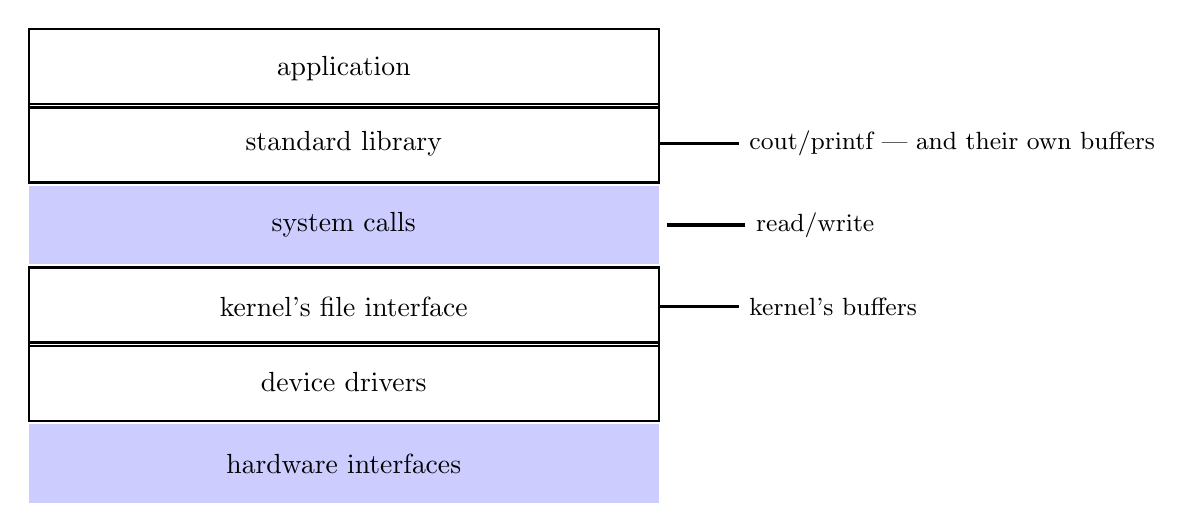
\begin{tikzpicture}
\tikzset{
    box/.style={draw,thick,minimum width=8cm,minimum height=1cm},
    thin box/.style={fill=blue!20,minimum width=8cm,minimum height=1cm,outer sep=1mm},
}
\begin{scope}[start chain=going below,node distance=-.75mm,every node/.style={on chain}]
\node[box] (application) {application};
\node[box] (library) {standard library};
\node[thin box] (syscalls) {system calls};
\node[box] (kernel file) {kernel's file interface};
\node[box] (device driver) {device drivers};
\node[thin box] (hardware) {hardware interfaces};
\end{scope}
\draw[very thick] (kernel file.east) -- ++(1cm,0cm) node[right,font=\small] {kernel's buffers};
\draw[very thick] (syscalls.east) -- ++(1cm,0cm) node[right,font=\small] {read/write};
\draw[very thick] (library.east) -- ++(1cm,0cm) node[right,font=\small] {cout/printf --- \myemph{and their own buffers}};
\end{tikzpicture}
\end{frame}

\begin{frame}{why the extra layer}
    \begin{itemize}
        \item better (but more complex to implement) interface:
            \begin{itemize}
            \item read line 
            \item formatted input (scanf, cin into integer, etc.)
            \item formatted output
            \end{itemize}
        \item less system calls (bigger reads/writes) sometimes faster
            \begin{itemize}
            \item buffering can combine multiple in/out library calls into one system call
            \end{itemize}
        \item more portable interface
            \begin{itemize}
            \item cin, printf, etc. defined by C and C++ standards
            \end{itemize}
    \end{itemize}
\end{frame}



\subsection{pipe blocking}

\begin{frame}[fragile,label=pipeAndBlocking]{pipe() and blocking}
\myemph{BROKEN} example:
\begin{lstlisting}[language=C++,style=small]
int pipe_fd[2];
if (pipe(pipe_fd) < 0)
    handle_error();
int read_fd = pipe_fd[0];
int write_fd = pipe_fd[1];
write(write_fd, some_buffer, some_big_size);
read(read_fd, some_buffer, some_big_size);
\end{lstlisting}
This is likely to \myemph{not terminate}. What's the problem?
\end{frame}

\subsection{waiting for more than one?}


\usetikzlibrary{arrows.meta,decorations.pathmorphing,fadings}

\begin{frame}[fragile,label=patternMultSnake]{pattern with multiple?}
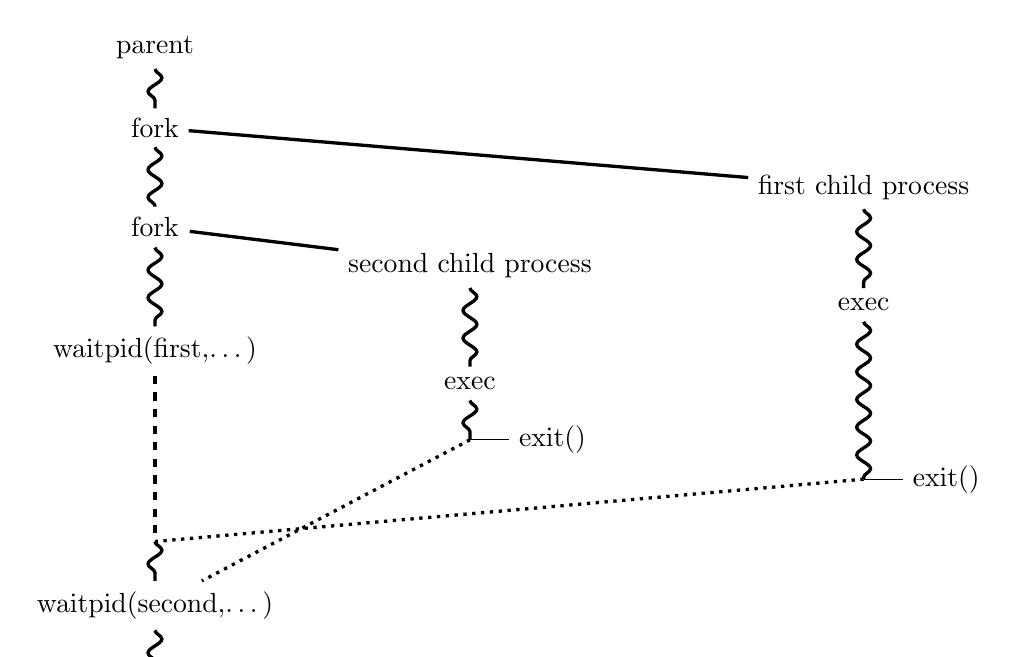
\begin{tikzpicture}
\tikzset{
    thread/.style={very thick,draw,decorate,decoration=snake},
    split/.style={very thick,draw},
    marker/.style={thin,draw},
}
\path[thread] (0, 0) --  (0, -.5);
\node[anchor=south] at (0,0) {parent};
\node[anchor=north] (fork mark 1) at (0, -.5) {fork};
\draw[thread] (fork mark 1) -- ++(0, -1) node[below] (fork mark 2) {fork};
\draw[thread] (fork mark 2.south) -- ++(0, -1) node[below] (wait 1 start) {waitpid(first,\ldots)};
\node (child 1 start) at (9, -1.5) {first child process};
\node (child 2 start) at (4, -2.5) {second child process};
\path[split] (fork mark 1) --  (child 1 start);
\path[split] (fork mark 2) --  (child 2 start);
\path[thread] (child 1 start.south) -- ++(0, -1) node[below] (exec 1) {exec};
\path[thread] (exec 1.south) -- ++(0, -2) coordinate (exec 1 done);
\path[marker] (exec 1 done) -- ++(.5, 0) node[right] {exit()};
\path[thread] (child 2 start.south) -- ++(0, -1) node[below] (exec 2) {exec};
\path[thread] (exec 2.south) -- ++ (0, -0.5) coordinate (exec 2 done);
\path[marker] (exec 2 done) -- ++(.5, 0) node[right] {exit()};
\path[split,dotted] (exec 1 done) -- (0, -6) coordinate (wait 1 done);;
\draw[very thick,dashed] (wait 1 start) -- (wait 1 done);
\draw[thread] (wait 1 done) -- ++(0, -.5) node[below] (wait 2 start) { waitpid(second,\ldots) };
\path[split,dotted] (exec 2 done) -- (wait 2 start);
\draw[overlay,thread] (wait 2 start.south) -- ++ (0, -2);
\end{tikzpicture}
\end{frame}



\subsection{POSIX and Unix}

\usetikzlibrary{calc}

\begin{frame}{this class: focus on Unix}
    \begin{itemize}
    \item Unix-like OSes will be our focus
    \item we have source code
    \item used to from 2150, etc.?
    \item have been around for a while
    \item xv6 imitates Unix
    \end{itemize}
\end{frame}

\begin{frame}{Unix history}
\vspace{-.5cm}
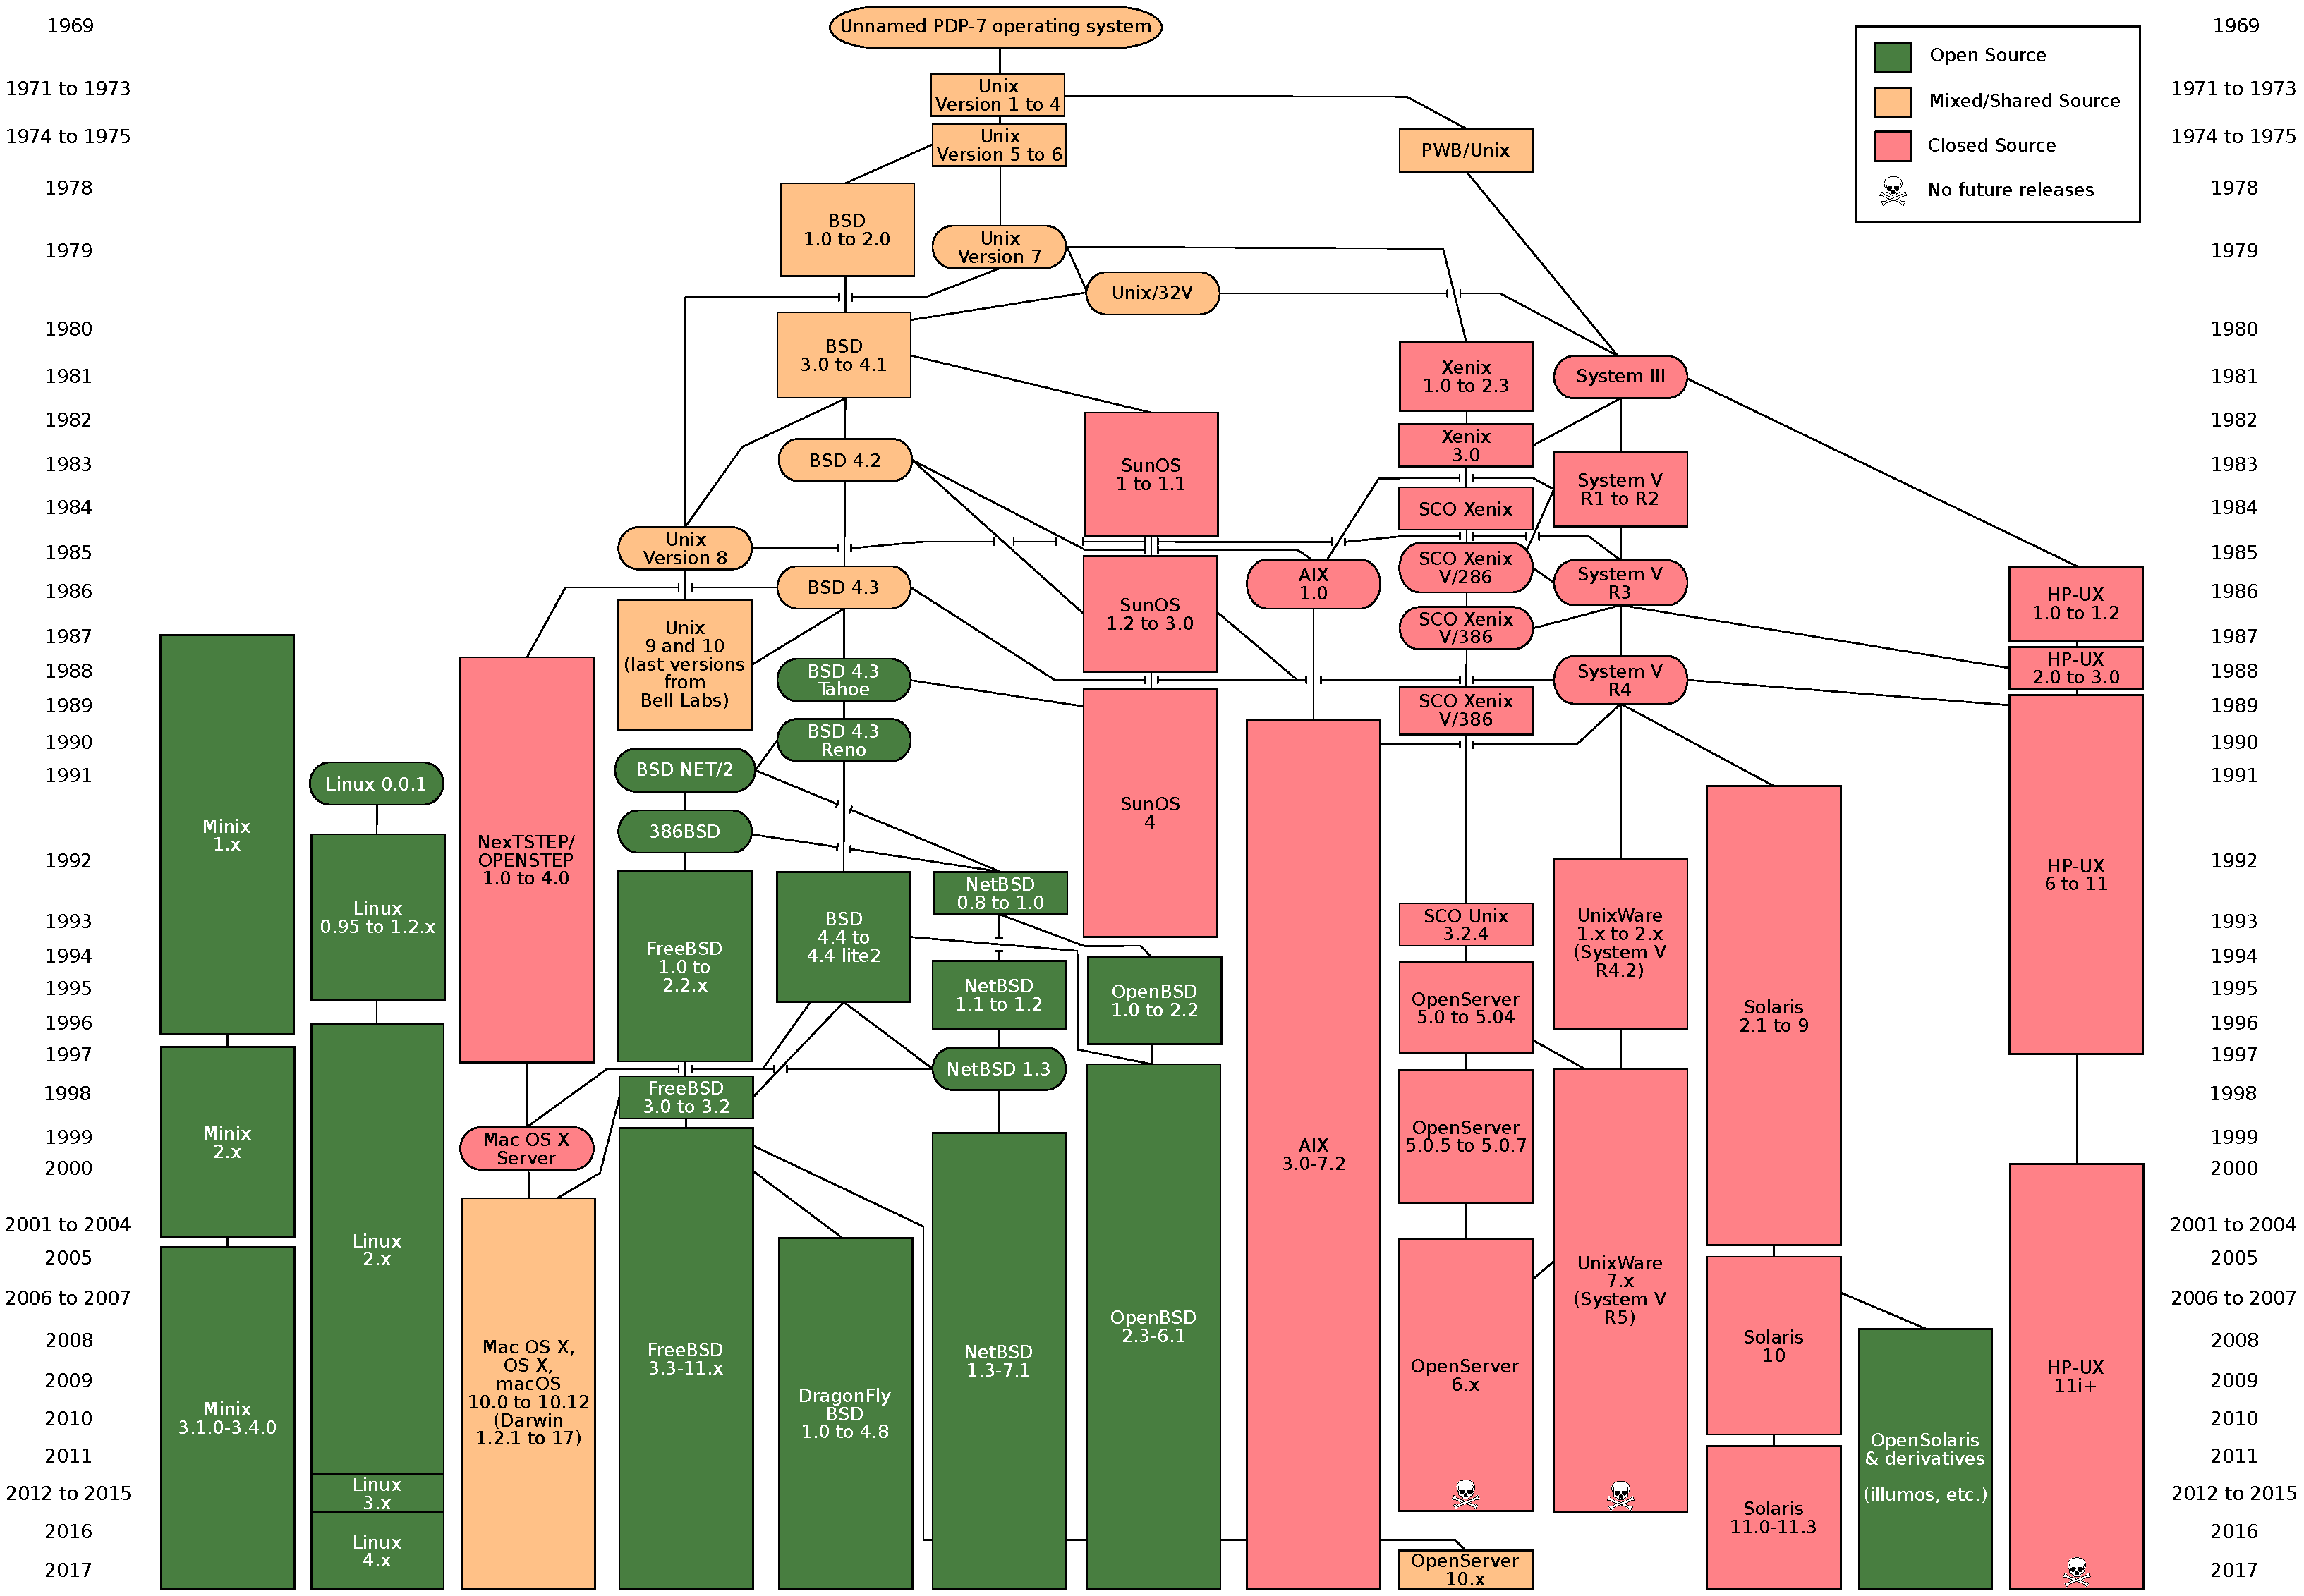
\includegraphics[height=0.9\textheight]{../unix-api/Unix_history-simple_en.pdf}
\imagecredit{image: Wikpedia/Eraserhead1+Infinity0+Sav\_vas}
\end{frame}

\begin{frame}{POSIX: standardized Unix}
\begin{itemize}
\item Portable Operating System Interface (POSIX) 
    \begin{itemize}
    \item ``standard for Unix''
    \end{itemize}
\item current version online: https://pubs.opengroup.org/onlinepubs/9699919799/
\item (almost) followed by most current Unix-like OSes
\item \ldots but OSes add extra features
\item \ldots and POSIX doesn't specify everything
\end{itemize}
\end{frame}

\begin{frame}{what POSIX defines}
\begin{itemize}
\item POSIX specifies the \myemph{library and shell interface}
    \begin{itemize}
    \item source code compatibility
    \end{itemize}
\item doesn't care what is/is not a system call\ldots
\item doesn't specify binary formats\ldots
\item idea: write applications for POSIX, recompile and run on all implementations
    \begin{itemize}
    \item this was a very important goal in the 80s/90s
    \item at the time, no dominant Unix-like OS (Linux was very immature)
    \end{itemize}
\end{itemize}
\end{frame}


\subsection{getpid}

\begin{frame}[fragile,label=getpid]{getpid}
\begin{lstlisting}[language=C++]
pid_t my_pid = getpid();
printf("my pid is %ld\n", (long) my_pid);
\end{lstlisting}
\end{frame}

\begin{frame}[fragile,label=ps]{process ids in ps}
\begin{Verbatim}
cr4bd@machine:~$ ps
  PID TTY          TIME CMD
14777 pts/3    00:00:00 bash
14798 pts/3    00:00:00 ps
\end{Verbatim}
\end{frame}


\subsection{read, write}

% FIXME: work through examples more


\begin{frame}<0>[fragile,label=readWrite]{read/write}
\begin{lstlisting}
ssize_t read(int fd, void *buffer, size_t count);
ssize_t write(int fd, void *buffer, size_t count);
\end{lstlisting}
\begin{itemize}
\item read/write \myemph<2>{up to \textit{count}} bytes to/from \textit{buffer}
\item returns number of bytes read/written or -1 on error
    \begin{itemize}
    \item ssize\_t is a signed integer type
    \item error code in \texttt{errno}
    \end{itemize}
\item read returning 0 means end-of-file (\textit{not an error})
\begin{itemize}
\item can read/write less than requested (end of file, broken I/O device, \ldots)
\end{itemize}
\end{itemize}
\end{frame}

\againframe<1>{readWrite}

\begin{frame}[fragile,label=readExample1]{read'ing one byte at a time}
\begin{lstlisting}[language=C++,style=small,morekeywords=ssize\_t,morekeywords=string]
string s;
ssize_t amount_read;
char c;
/* cast to void * not needed in C */
while ((amount_read = read(STDIN_FILENO, (void*) &c, 1)) > 0) {
    /* amount_read must be exactly 1 */
    s += c;
}
if (amount_read == -1) {
    /* some error happened */
    perror("read"); /* print out a message about it */
} else if (amount_read == 0) {
    /* reached end of file */
}
\end{lstlisting}
\end{frame}



\begin{frame}[fragile,label=writeExample]{write example}
\begin{lstlisting}[language=C++,style=small]
/* cast to void * optional in C */
write(STDOUT_FILENO, (void *) "Hello, World!\n", 14);
\end{lstlisting}
\end{frame}





\subsection{aside: environment variables}

\begin{frame}[fragile,label=envVarsPrintenv]{aside: environment variables (1)}
\begin{itemize}
\item key=value pairs associated with every process:
\end{itemize}
\begin{Verbatim}[fontsize=\fontsize{8}{9}\selectfont,commandchars=\\\{\}]
$ \textbf{printenv}
MODULE_VERSION_STACK=3.2.10
MANPATH=:/opt/puppetlabs/puppet/share/man
XDG_SESSION_ID=754
HOSTNAME=labsrv01 
SELINUX_ROLE_REQUESTED=
TERM=screen
SHELL=/bin/bash 
HISTSIZE=1000 
SSH_CLIENT=128.143.67.91 58432 22 
SELINUX_USE_CURRENT_RANGE=
QTDIR=/usr/lib64/qt-3.3
OLDPWD=/zf14/cr4bd
QTINC=/usr/lib64/qt-3.3/include
SSH_TTY=/dev/pts/0
QT_GRAPHICSSYSTEM_CHECKED=1
USER=cr4bd
LS_COLORS=rs=0:di=01;34:ln=01;36:mh=00:pi=40;33:so=01;35:do=01;35:bd=40;33;01:cd=40;33;01:or=40;31;01:mi=01;05;37;41:su=37;41:sg=30;43:ca=30;41:tw=30;42:ow=34;42:st=37;44:ex=01;32:*.tar=01;31:*.tgz=01;31:*.arc=01;31:*.arj=01;31:*.taz=01;31:*.lha=01;31:*.lz4=01;31:*.lzh=01;31:*.lzma=01;31:*.tlz=01;31:*.txz=01;31:*.tzo=01;31:*.t7z=01;31:*.zip=01;31:*.z=01;31:*.Z=01;31:*.dz=01;31:*.gz=01;31:*.lrz=01;31:*.lz=01;31:*.lzo=01;31:*.xz=01;31:*.bz2=01;31:*.bz=01;31:*.tbz=01;31:*.tbz2=01;31:*.tz=01;31:*.deb=01;31:*.rpm=01;31:*.jar=01;31:*.war=01;31:*.ear=01;31:*.sar=01;31:*.rar=01;31:*.alz=01;31:*.ace=01;31:*.zoo=01;31:*.cpio=01;31:*.7z=01;31:*.rz=01;31:*.cab=01;31:*.jpg=01;35:*.jpeg=01;35:*.gif=01;35:*.bmp=01;35:*.pbm=01;35:*.pgm=01;35:*.ppm=01;35:*.tga=01;35:*.xbm=01;35:*.xpm=01;35:*.tif=01;35:*.tiff=01;35:*.png=01;35:*.svg=01;35:*.svgz=01;35:*.mng=01;35:*.pcx=01;35:*.mov=01;35:*.mpg=01;35:*.mpeg=01;35:*.m2v=01;35:*.mkv=01;35:*.webm=01;35:*.ogm=01;35:*.mp4=01;35:*.m4v=01;35:*.mp4v=01;35:*.vob=01;35:*.qt=01;35:*.nuv=01;35:*.wmv=01;35:*.asf=01;35:*.rm=01;35:*.rmvb=01;35:*.flc=01;35:*.avi=01;35:*.fli=01;35:*.flv=01;35:*.gl=01;35:*.dl=01;35:*.xcf=01;35:*.xwd=01;35:*.yuv=01;35:*.cgm=01;35:*.emf=01;35:*.axv=01;35:*.anx=01;35:*.ogv=01;35:*.ogx=01;35:*.aac=01;36:*.au=01;36:*.flac=01;36:*.mid=01;36:*.midi=01;36:*.mka=01;36:*.mp3=01;36:*.mpc=01;36:*.ogg=01;36:*.ra=01;36:*.wav=01;36:*.axa=01;36:*.oga=01;36:*.spx=01;36:*.xspf=01;36:
MODULE_VERSION=3.2.10
MAIL=/var/spool/mail/cr4bd
PATH=/zf14/cr4bd/.cargo/bin:/zf14/cr4bd/bin:/usr/lib64/qt-3.3/bin:/usr/local/bin:/usr/bin:/usr/local/sbin:/usr/sbin:/opt/puppetlabs/bin:/usr/cs/contrib/bin:.
PWD=/zf14/cr4bd
LANG=en_US.UTF-8
MODULEPATH=/sw/centos/Modules/modulefiles:/sw/linux-any/Modules/modulefiles
LOADEDMODULES=
KDEDIRS=/usr
\textbf{\ldots}
_=/usr/bin/printenv
\end{Verbatim}
\end{frame}

\begin{frame}[fragile,label=envVarsFuncs]{aside: environment variables (2)}
\begin{itemize}
\item environment variable library functions:
    \begin{itemize}
    \item \texttt{getenv("KEY")} $\rightarrow$ \textit{value}
    \item \texttt{putenv("KEY=\textit{value}")} (sets KEY to \textit{value})
    \item \texttt{setenv("KEY", "value")} (sets KEY to \textit{value})
    \end{itemize}
\item {\fontsize{12}{13}\texttt{int execve(char *path, char **argv, char **envp)}}
\begin{lstlisting}[language=C++,style=small]
    char *envp[] = { "KEY1=value1", "KEY2=value2", NULL };
    char *argv[] = { "somecommand", "some arg", NULL };
    execve("/path/to/somecommand", argv, envp);
\end{lstlisting}
\item normal exec versions --- keep same environment variables
\end{itemize}
\end{frame}

\begin{frame}[fragile,label=envVarsUse]{aside: environment variables (3)}
\begin{itemize}
\item interpretation up to programs, but common ones\ldots
\vspace{.5cm}
\item \texttt{PATH=/bin:/usr/bin} 
    \begin{itemize}
    \item to run a program `foo', look for an executable in \texttt{/bin/foo}, then \texttt{/usr/bin/foo}
    \end{itemize}
\item \texttt{HOME=/zf14/cr4bd} 
    \begin{itemize}
    \item current user's home directory is `/zf14/cr4bd'
    \end{itemize}
\item \texttt{TERM=screen-256color} 
    \begin{itemize}
    \item your output goes to a `screen-256color'-style terminal
    \end{itemize}
\item \ldots
\end{itemize}
\end{frame}


\subsection{wait for mutliple}

\begin{frame}[fragile,label=typicalPatternMultiple1]{multiple processes?}
\begin{lstlisting}[language=C++,style=small]
while (...) {
    pid = fork();
    if (pid == 0) {
        exec ...
    } else if (pid > 0) {
        pids.push_back(pid);
    }
}

/* retrieve exit statuses in order */
for (pid_t pid : pids) {
    waitpid(pid, ...); 
    ...
}
\end{lstlisting}
\end{frame}
 

\subsection{wait for all}

\begin{frame}[fragile,label=waitForAny]{waiting for all children}
\begin{lstlisting}[
    language=C++,
    style=smaller,
    moredelim={**[is][\btHL<2|handout:0>]{@2}{2@}},
]
#include <sys/wait.h>
...
  while (true) {
    pid_t child_pid = waitpid(-1, &status, 0);
    if (child_pid == (pid_t) -1) {
      if (errno == ECHILD) {
        /* no child process to wait for */
        break;
      } else {
        /* some other error */
      }
    }
    /* handle child_pid exiting */
  }
\end{lstlisting}
\end{frame}


\subsection{wait for all (alt)}


\begin{frame}[fragile,label=typicalPatternMultiple2]{multiple processes?}
\begin{lstlisting}[language=C++,style=small]
while (...) {
    pid = fork();
    if (pid == 0) {
        exec ...
    } else if (pid > 0) {
        pids.push_back(pid);
    }
}

/* retrieve exit statuses as processes finish */
while ((pid = waitpid(-1, ...)) != -1) {
    handleProcessFinishing(pid);
}
\end{lstlisting}
\end{frame}



\subsection{waitpid WNOHANG}


\begin{frame}[fragile,label=waitNoHang]{`waiting' without waiting}
\begin{lstlisting}[
    language=C++,
    style=smaller,
    moredelim={**[is][\btHL<2|handout:0>]{@2}{2@}},
]
#include <sys/wait.h>
...
  pid_t return_value = waitpid(child_pid, &status, WNOHANG);
  if (return_value == (pid_t) 0) {
    /* child process not done yet */
  } else if (child_pid == (pid_t) -1) {
    /* error */
  } else {
    /* handle child_pid exiting */
  }
\end{lstlisting}
\end{frame}


\subsection{parent and child}
\begin{frame}{parent and child processes}
\begin{itemize}
    \item every process (but process id 1) has a \textit{parent process} (\texttt{getppid()})
    \item this is the process that can wait for it
    \item creates tree of processes (Linux \texttt{pstree} command):
\end{itemize}
    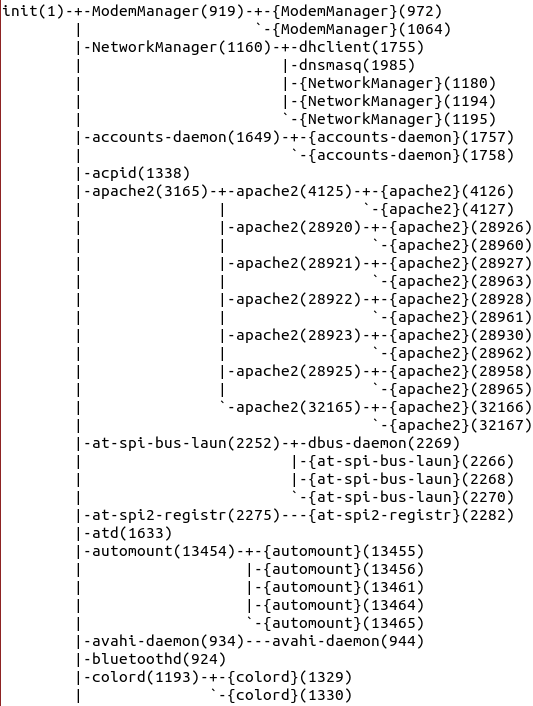
\includegraphics[height=0.6\textheight]{../unix-api/process-tree}
    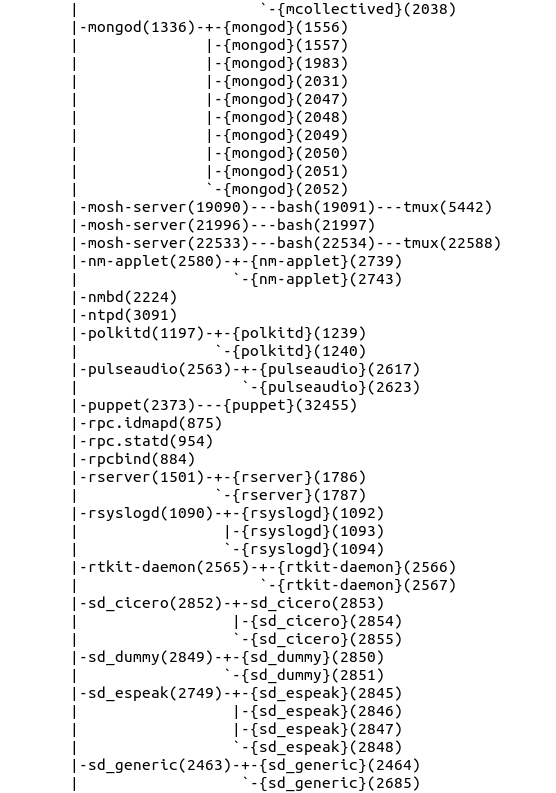
\includegraphics[height=0.6\textheight]{../unix-api/process-tree2}
\end{frame}

\begin{frame}{parent and child questions\ldots}
\begin{itemize}
    \item what if parent process exits before child?
        \begin{itemize}
        \item child's parent process becomes process id 1 (typically called \textit{init})
        \end{itemize}
    \item what if parent process never \texttt{waitpid()}s {\small (or equivalent)} for child?
        \begin{itemize}
        \item child process stays around as a ``zombie'' 
        \item can't reuse pid in case parent wants to use \texttt{waitpid()}
        \end{itemize}
    \item what if non-parent tries to \texttt{waitpid()} for child?
        \begin{itemize}
        \item waitpid fails
        \end{itemize}
\end{itemize}
\end{frame}




\section{partial reads and writes}
\subsection{partial reads and read error checking}

\begin{frame}[fragile,label=readExample2]{read'ing a fixed amount}
\begin{lstlisting}[language=C++,style=small,morekeywords=ssize\_t]
ssize_t offset = 0;
const ssize_t amount_to_read = 1024;
char result[amount_to_read];
do {
    /* cast to void * optional in C */
    ssize_t amount_read = 
        read(STDIN_FILENO,
             (void *) (result + offset),
             amount_to_read - offset);
    if (amount_read < 0) {
        perror("read"); /* print error message */
        ... /* abort??? */
    } else {
        offset += amount_read;
    }
} while (offset != amount_to_read && amount_read != 0);
\end{lstlisting}
\end{frame}

\begin{frame}{partial reads}
\begin{itemize}
    \item on regular file: read reads what you request
    \item but otherwise: usually gives you what's known to be available
        \begin{itemize}
            \item after waiting for something to be available
        \end{itemize}
    \vspace{.5cm}
    \item<2-> reading from network --- what's been received
    \item<2-> reading from keyboard --- what's been typed
\end{itemize}
\end{frame}

\subsection{partial writes and write error checking}

\begin{frame}[fragile,label=writeExampleErrorChecking]{write example (with error checking)}
\begin{lstlisting}[language=C++,style=small,morekeywords=ssize\_t]
const char *ptr = "Hello, World!\n";
ssize_t remaining = 14;
while (remaining > 0) {
    /* cast to void * optional in C */
    ssize_t amount_written = write(STDOUT_FILENO,
                                   ptr,
                                   remaining);
    if (amount_written < 0) {
        perror("write"); /* print error message */
        ... /* abort??? */
    } else {
        remaining -= amount_written;
        ptr += amount_written;
    }
}
\end{lstlisting}
\end{frame}

\begin{frame}{partial writes}
\begin{itemize}
    \item usually only happen on error or interruption
        \begin{itemize}
        \item but can request ``non-blocking''
        \item (interruption: via \textit{signal})
        \end{itemize}
    \item \textit{usually}: write \myemph{waits until it completes}
        \begin{itemize}
        \item = until remaining part fits in buffer in kernel
        \item does not mean data was sent on network, shown to user yet, etc.
        \end{itemize}
\end{itemize}
\end{frame}


\subsection{kernel buffering}

\usetikzlibrary{arrows.meta,chains,shapes}

\begin{frame}{kernel buffering (reads)}
\begin{tikzpicture}
\tikzset{
    >=Latex,
    component box/.style={draw,thick,minimum width=10cm,minimum height=1cm,align=center},
    component box big/.style={component box,minimum height=2.5cm},
    component box small/.style={component box,minimum width=4cm},
    subcomponent box/.style={draw,thick,minimum width=2cm,align=center,font=\small},
    event line/.style={draw,ultra thick},
    event box/.style={draw,thick,fill=white,inner sep=0.25mm,font=\small, align=center},
    number box A/.style={draw=blue,thick,fill=blue!10,ellipse,font=\small,inner sep=0.1mm},
    number box A alt/.style={draw=blue,thick,dotted,fill=blue!5,ellipse,font=\small,inner sep=0.1mm,
            alt=<4>{draw=red,fill=red!10}},
    number box B/.style={draw=green,thick,fill=green!10,ellipse,font=\small,inner sep=0.1mm},
}
\node[component box] (process) {program};
\node[component box big,anchor=north] (os) at ([yshift=-2cm]process.south) {operating system \\ ~ \\ ~};
\node[component box small,anchor=north east] (keyboard) at ([xshift=-.5cm,yshift=-1.5cm]os.south) {keyboard};
\node[component box small,anchor=north west] (disk) at ([xshift=.5cm,yshift=-1.5cm]os.south) {disk};
\begin{visibleenv}<2->
\draw[event line,->] (keyboard.north) -- (os.south -| keyboard.north) node[midway,event box] (kp event){keypress happens, read};
\node[number box A,anchor=east] (kp event number) at (kp event.north west) {1};
\begin{visibleenv}<4->
    \node[number box A alt,anchor=east] at ([xshift=-.5cm,yshift=.1cm]kp event number.west) {2};
    \node[font=\small,anchor=east,inner sep=0.25mm] at (kp event number.west) {or};
\end{visibleenv}
\node[anchor=south,subcomponent box] (keyboard buffer)  at (os.south -| keyboard.north) {buffer: keyboard input \\ waiting for program};
\end{visibleenv}
\begin{visibleenv}<3->
    \draw[event line,->] ([xshift=-4cm]process.south) -- ([xshift=-4cm]os.north) node[midway,event box,xshift=-1cm] (read ev) {read char \\ from terminal};
\node[number box A,anchor=east] (read ev number) at (read ev.north west) {2};
\begin{visibleenv}<4->
    \node[number box A alt,anchor=east] at ([xshift=-.5cm,yshift=.1cm]read ev number.west) {1};
    \node[font=\small,anchor=east,inner sep=0.25mm] at (read ev number.west) {or};
\end{visibleenv}
    \draw[event line,<-] ([xshift=-2cm]process.south) -- ([xshift=-2cm]os.north) node[midway,event box,xshift=-.5cm] (from buf ev) {\ldots via buffer};
\node[number box A,anchor=east] at (from buf ev.north west) {3};
\end{visibleenv}
\begin{visibleenv}<5->
\draw[event line,->] ([xshift=1cm]process.south) -- ([xshift=1cm]os.north) node[midway,event box,xshift=0cm] (read file ev)  {read char \\ from file};
\node[number box B,anchor=east] at (read file ev.north west) {1};
\end{visibleenv}
\begin{visibleenv}<6->
\draw[event line,->] (disk.north) -- (os.south -| disk.north) node[midway,event box] (xfer disk ev) {read \textit{block} of data from disk};
\node[number box B,anchor=east] at (xfer disk ev.north west) {2};
\node[anchor=south,subcomponent box] at (os.south -| disk.north) {buffer: recently read \\ data from disk};
    \draw[event line,<-] ([xshift=4cm]process.south) -- ([xshift=4cm]os.north) node[midway,event box,xshift=0cm] (from disk buffer ev) {\ldots via buffer};
\node[number box B,anchor=east] at (from disk buffer ev.north west) {3};
\end{visibleenv}
\end{tikzpicture}
\end{frame}

\begin{frame}{kernel buffering (writes)}
\begin{tikzpicture}
\tikzset{
    >=Latex,
    component box/.style={draw,thick,minimum width=10cm,minimum height=1cm,align=center},
    component box big/.style={component box,minimum height=2.25cm},
    component box small/.style={component box,minimum width=4cm},
    subcomponent box/.style={draw,thick,minimum width=2cm,align=center,font=\small},
    event line/.style={draw,ultra thick},
    event box/.style={draw,thick,fill=white,inner sep=0.25mm,font=\small, align=center},
}
\node[component box] (process) {program};
\node[component box big,anchor=north] (os) at ([yshift=-2cm]process.south) {operating system \\ ~ \\ ~};
\node[component box small,anchor=north east] (network) at ([xshift=-.5cm,yshift=-1.5cm]os.south) {network};
\node[component box small,anchor=north west] (disk) at ([xshift=.5cm,yshift=-1.5cm]os.south) {disk};
\begin{visibleenv}<3->
\draw[event line,<-] (keyboard.north) -- (os.south -| keyboard.north) node[midway,event box] {(when ready) \\ send data};
\node[anchor=south,subcomponent box] (keyboard buffer)  at (os.south -| keyboard.north) {buffer: output \\ waiting for network};
\end{visibleenv}
\begin{visibleenv}<2->
\draw[event line,->] ([xshift=-4cm]process.south) -- ([xshift=-4cm]os.north) node[midway,event box,xshift=0cm] {print char \\ to remote machine};
\end{visibleenv}
\begin{visibleenv}<4->
\draw[event line,->] ([xshift=1cm]process.south) -- ([xshift=1cm]os.north) node[midway,event box,xshift=0cm] {write char \\ to file};
\end{visibleenv}
\begin{visibleenv}<5->
\draw[event line,<-] (disk.north) -- (os.south -| disk.north) node[midway,event box] {(when ready) \\ write \textit{block} of data from disk};
\node[anchor=south,subcomponent box] at (os.south -| disk.north) {buffer: data waiting \\ to be written on disk};
\end{visibleenv}
\end{tikzpicture}
\end{frame}

\begin{frame}{read/write operations}
\begin{itemize}
\item read()/write(): move data into/out of buffer
\item possibly wait if buffer is empty (read)/full (write)
\vspace{.5cm}
\item actual I/O operations --- wait for device to be ready
    \begin{itemize}
    \item trigger process to stop waiting if needed
    \end{itemize}
\end{itemize}
\end{frame}


\subsection{open}
\begin{frame}{filesystem abstraction}
\begin{itemize}
\item regular files --- named collection of bytes
    \begin{itemize}
    \item also: size, modification time, owner, access control info, \ldots
    \end{itemize}
\item directories --- folders containing files and directories
    \begin{itemize}
    \item hierarchical naming: \texttt{/net/zf14/cr4bd/fall2018/cs4414}
    \item \textit{mostly} contains regular files or directories
    \end{itemize}
\end{itemize}
\end{frame}

\begin{frame}[fragile,label=openExample]{open}
\begin{lstlisting}[
    language=C++,
    moredelim={**[is][\btHL<1-|handout:1->]{@1}{1@}},
]
int open(const char *path, int flags);
int open(const char *path, int flags, int mode);
...

int read_fd = open("dir/file1", O_RDONLY);
int write_fd = open("/other/file2",
        O_WRONLY | O_CREAT | O_TRUNC, 0666);
int rdwr_fd = open("file3", O_RDWR);
\end{lstlisting}
\end{frame}

\begin{frame}[fragile,label=openExplainPath]{open}
\begin{lstlisting}[
    language=C++,
    moredelim={**[is][\btHL<1-|handout:1->]{@1}{1@}},
]
int open(const char *@1path1@, int flags);
int open(const char *@1path1@, int flags, int mode);
\end{lstlisting}
\begin{itemize}
\item path = filename
\item e.g. \texttt{"/foo/bar/file.txt"}
    \begin{itemize}
    \item \texttt{file.txt} in 
    \item directory \texttt{bar} in
    \item directory \texttt{foo} in 
    \item ``the root directory''
    \end{itemize}
\item e.g. \texttt{"quux/other.txt}
    \begin{itemize}
    \item \texttt{other.txt} in 
    \item directory \texttt{quux} in
    \item ``the current working directory'' (set with \texttt{chdir()})
    \end{itemize}
\end{itemize}
\end{frame}

\begin{frame}[fragile,label=openExplainFDs]{open: file descriptors}
\begin{lstlisting}[
    language=C++,
    moredelim={**[is][\btHL<1-|handout:1->]{@1}{1@}},
]
@1int1@ open(const char *path, int flags);
@1int1@ open(const char *path, int flags, int mode);
\end{lstlisting}
\begin{itemize}
\item return value = \myemph{file descriptor} {\small (or -1 on error)}
\item index into table of \textit{open file descriptions} for each process
\item used by system calls that deal with open files
\end{itemize}
\end{frame}



\subsection{Unix: everything is a file}

\usetikzlibrary{arrows.meta,chains}

\begin{frame}{POSIX: everything is a file}
\begin{itemize}
\item the file: one interface for
    \begin{itemize}
    \item devices (terminals, printers, \ldots)
    \item regular files on disk
    \item networking (sockets)
    \item local interprocess communication (pipes, sockets)
    \end{itemize}
    \vspace{.5cm}
    \item basic operations: open(), read(), write(), close()
\end{itemize}
\end{frame}


\section{pipe exercise (partial reads)}

\begin{frame}<1>[fragile,label=pipeExtraEx2]{exercise}
\vspace{-.25cm}
\begin{lstlisting}[language=C++,basicstyle=\tt\fontsize{9.5}{10.5}\selectfont]
int pipe_fds[2]; pipe(pipe_fds);
pid_t p = fork();
if (p == 0) {
  close(pipe_fds[0]);
  for (int i = 0; i < 10; ++i) {
    char c = '0' + i;
    write(pipe_fds[1], &c, 1);
  }
  exit(0);
}
close(pipe_fds[1]);
char buffer[10];
ssize_t count = read(pipe_fds[0], buffer, 10);
for (int i = 0; i < count; ++i) {
  printf("%c", buffer[i]);
}
\end{lstlisting}
Which of these are possible outputs {\small (if pipe, read, write, fork don't fail)}?
\begin{tabular}{lll}
A. \texttt{0123456789} & B. \texttt{0} & C. (nothing) \\
\myemph<2>{D.} A and B & E. A and C & F. A, B, and C \\
\end{tabular}
\end{frame}

\iftoggle{heldback}{}{\againframe<2>{pipeExtraEx2}}

\begin{frame}<0>[fragile,label=pipeExtraEx2More]{empirical evidence}
\begin{Verbatim}
      8 0
    374 01
    210 012
     30 0123
     12 01234
      3 012345
      1 0123456
      2 01234567
      1 012345678
    359 0123456789
\end{Verbatim}
\end{frame}

\iftoggle{heldback}{}{\againframe<2>{pipeExtraEx2More}}

\begin{frame}{partial reads}
\begin{itemize}
\item read returning 0 always means end-of-file
    \begin{itemize}
    \item by default, read always waits \textit{if no input available yet}
    \item but can set read to return \textit{error} instead of waiting
    \end{itemize}
\item read can return less than requested if not available
    \begin{itemize}
        \item e.g. child hasn't gotten far enough
    \end{itemize}
\end{itemize}
\end{frame}
 % FIXME: cut?

\section{pipe: closing?}
\begin{frame}{pipe: closing?}
    \begin{itemize}
    \item if all write ends of pipe are closed
        \begin{itemize}
        \item can get end-of-file (read() returning 0) on read end
        \item exit()ing closes them
        \end{itemize}
    \item $\rightarrow$ close write end when not using
    \vspace{.5cm}
    \item generally: limited number of file descriptors per process
    \item $\rightarrow$ good habit to close file descriptors not being used
    \item (but probably didn't matter for read end of pipes in example)
    \end{itemize}
\end{frame}


\subsection{dup2 exercise}
\begin{frame}[fragile,label=dup2ex]{dup2 exercise}
\begin{itemize}
\item recall: \texttt{dup2(old\_fd, new\_fd)}
\end{itemize}
\begin{lstlisting}[language=C,style=small]
int fd = open("output.txt", O_WRONLY | O_CREAT, 0666);
write(STDOUT_FILENO, "A", 1);
dup2(fd, STDOUT_FILENO);
pid_t pid = fork();
if (pid == 0) { /* child: */
    dup2(STDOUT_FILENO, fd); write(fd, "B", 1);
} else {
    write(STDOUT_FILENO, "C", 1);
}
\end{lstlisting}
Which outputs are possible?\\\small
\begin{tabular}{ll}
A. stdout: ABC ; output.txt: empty & D. stdout: A ; output.txt: BC \\
B. stdout: AC ; output.txt: B &  E. more? \\
C. stdout: A ; output.txt: CB \\
\end{tabular}
\end{frame}

